\documentclass{article}

\usepackage{corl_2026} % Anonymized submission mode.
% \usepackage[final]{corl_2026} % Camera-ready.
% \usepackage[preprint]{corl_2026} % Preprint: shows authors.

\usepackage{amsmath}
\usepackage{graphicx}
\usepackage{booktabs}

\graphicspath{{../figures/paper/}}

% Draft v0.6, 2026-08-18. Canonical source (docs/paper.md frozen at v0.4).
% Status: main grid final (5 seeds); guarded column and hardware calibration
% (App. D) in progress. Full lab record in docs/findings.md.

\title{A Retroactive Contact Channel for Behavior Cloning on Low-Cost Arms}

% Authors visible only under [final]/[preprint].
\author{
  Luai Abuelsamen\\
  University of California, Berkeley\\
  \texttt{luai\_abuelsamen@berkeley.edu}
}

\begin{document}
\maketitle

%===============================================================================

\begin{abstract}
Low-cost servo arms ship without force sensing, and standard imitation-learning stacks observe joint positions only, so learned policies close the gripper open-loop against contact. For logs that record synchronized joint-position commands and measured positions, the servo tracking error $\delta = a[t{-}1] - s[t]$ is a contact proxy that can be computed retrospectively, and current stacks discard it. In a pre-registered six-design study at 280 demonstrations on a simulated force-critical task (5 seeds $\times$ 100 paired episodes), every observation that carries this channel outperforms the channel-free base, while predicting $\delta$ as an auxiliary training target does not. The strongest design appends a free-motion-compensated residual, the \emph{lag excess}, and is the only one to outperform an action-history baseline at our pre-declared seed resolution (26.6\% success versus 13.8\%; 95\% CI on the difference $[+2.8, +22.6]$). On 546 episodes across 16 public teleoperation datasets, the pre-registered prediction that successful grasps carry higher $\delta$ fails: under the frozen outcome proxy, high $\delta$ at grasp time is associated with failure, consistent with operators forcing jammed grasps. Code and data at [URL].
\end{abstract}

\keywords{Imitation Learning, Force Estimation, Low-Cost Manipulation}

%===============================================================================

\begin{figure}[t]
  \centering
  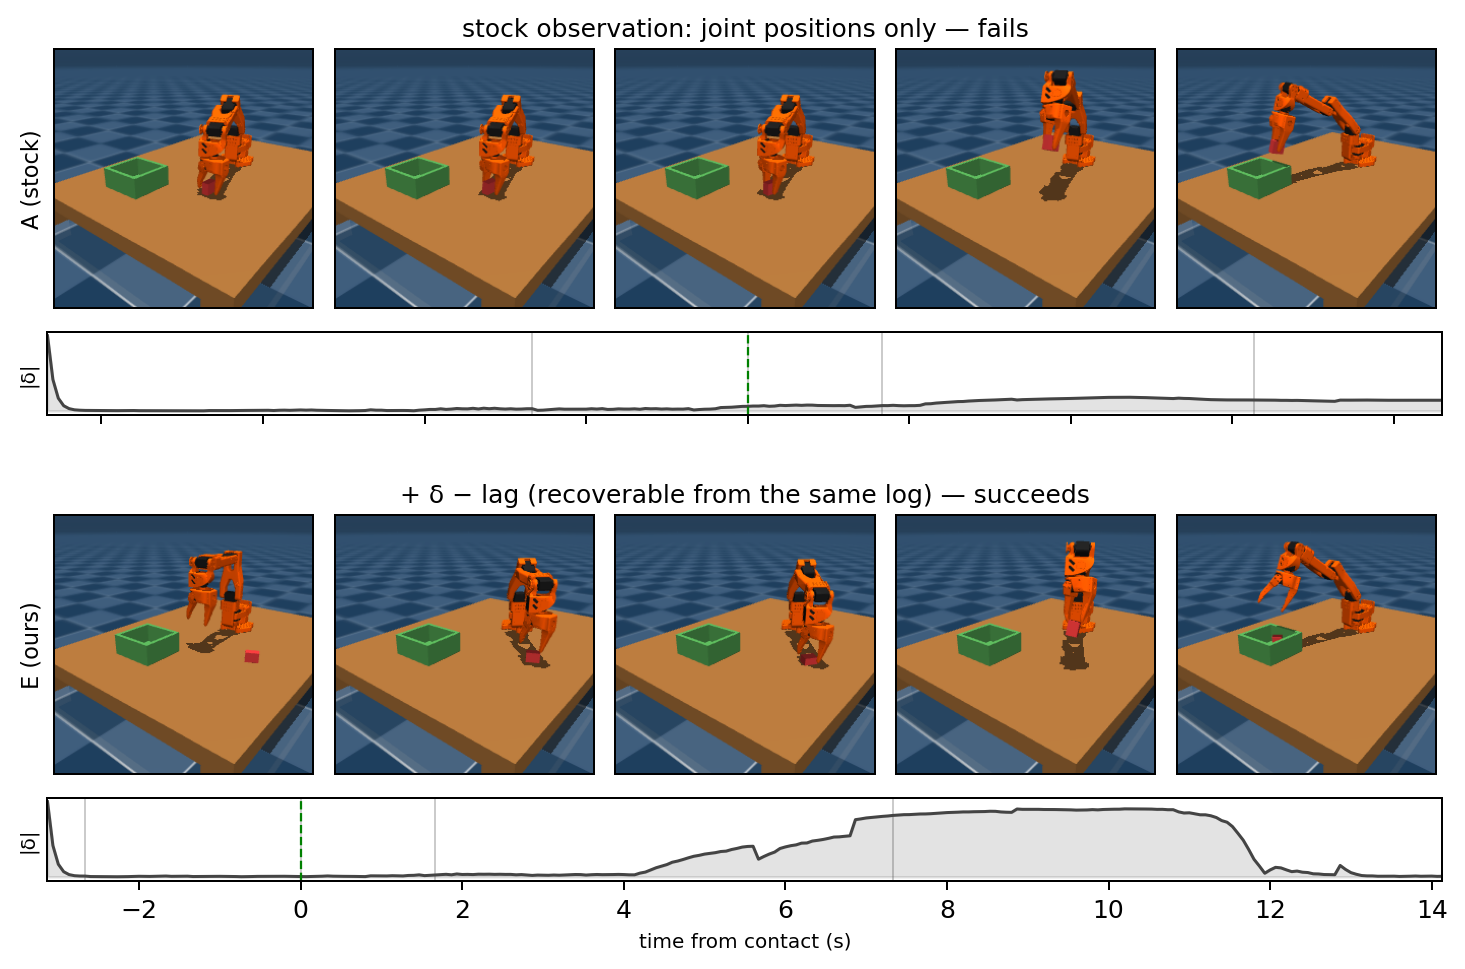
\includegraphics[width=0.9\linewidth]{fig_teaser.png}
  \caption{Two policies, identical scene and data budget (280
  demonstrations). Top: the stock observation (joint positions only)
  reaches, grips, and releases without lifting. Bottom: the same network
  with the contact channel appended to its state vector places the block.
  The traces plot $|\delta|$ on the jaw joint; the contact plateau in both
  is the signal the top policy never receives. Both are computed from the
  same log fields.}
  \label{fig:teaser}
\end{figure}

\section{Introduction}
\label{sec:intro}

Low-cost servo arms and open imitation-learning stacks have made
manipulation research broadly accessible: ACT on ALOHA-class
hardware~\citep{zhao2023act}, diffusion policies~\citep{chi2023diffusion},
and the LeRobot ecosystem~\citep{cadene2024lerobot} with its VLA
descendants~\citep{kim2024openvla, black2024pi0, shukor2025smolvla,
nvidia2025groot} all train behavior cloning on teleoperated
demonstrations, and all share one proprioceptive default: the current
measured joint positions, one timestep, nothing else
(Sec.~\ref{sec:related}).

This default fails at contact. The arms carry no force or tactile sensors,
so a position-only policy cannot distinguish a seated grasp from an empty
close: crushed objects, unseated grips, drops during transport. The
omission is not for lack of signal. The servos are proportional position
controllers, so when the jaw meets an object the measured position stalls
while the command deepens, and the gap reflects the servo's deflection
under load. The authors of ACT state the physics directly: force ``is
implicitly defined by the difference between'' leader and follower
positions~\citep{zhao2023act}, and a recent intervention study shows that
removing this discrepancy signal from ACT's action labels breaks
force-critical tasks~\citep{wong2026beyond}. Yet the stack keeps one
operand of that subtraction in the action labels and never provides the
difference as an observation; the LeRobot Feetech driver reads only
\texttt{Present\_Position} into the state vector, and the reference ACT
implementation raises on \texttt{n\_obs\_steps != 1}~\citep{cadene2024lerobot}.

The channel has a property no current- or torque-based estimator shares:
it is recoverable retroactively. Wherever a recorded dataset's
\texttt{action} field holds joint-position commands synchronized with
\texttt{observation.state} in a common frame,
$\delta = a[t{-}1] - s[t]$ can be computed after the fact; 16 of the 20
public datasets we targeted passed our frozen inclusion gates
(Sec.~\ref{sec:corpus}, which also owns the caveats on action semantics).
The same signal supports runtime enforcement from bus telemetry alone
(Sec.~\ref{sec:guard}).

We ask what a small-data policy must observe to use this channel, and
compare six observation designs that differ only in which function of the
logged pair enters the state vector. The best tested form is the
\emph{lag excess} $e[t] = \delta[t] - \hat{K} r[t]$, which subtracts a
per-joint free-motion following-lag model fit on the jaw-open frames of
the training demonstrations, label-free and frozen before training
(Sec.~\ref{sec:formulation}; implementation details in
App.~\ref{app:impl}).

Three results are established at our pre-declared seed resolution
(Sec.~\ref{sec:grid}). Channel-bearing observation beats channel-free in
every input form. The tested auxiliary-prediction baseline recovers none
of the direct-input gain: the same information moves performance as an
input and not as a training target. And the lag excess is the only tested
design to beat raw action history (26.6\% vs.\ 13.8\%, CI
$[+2.8, +22.6]$); whether its edge over raw $\delta$ comes from the
subtraction is not resolved at this budget, so we present it as the
recommended instantiation, not a finding about the subtraction itself. On
the public corpus, a pre-registered prediction fails: high $\delta$ at
grasp time accompanies failed grasps, and the traces attribute this to
operators over-commanding at contact (Sec.~\ref{sec:corpus}). A 40-line guard on the same telemetry removes
96\% of simulated crush events without retraining (Sec.~\ref{sec:guard}).

We summarize our contributions below:
\begin{itemize}
  \item Characterization of servo tracking error as a contact/load proxy
  with a validity envelope and a resolution-vs-margin design rule
  (Sec.~\ref{sec:channel}, \ref{sec:validity}).
  \item A pre-registered six-design observation study at 280
  demonstrations: observe the channel; predicting it does not substitute
  (Sec.~\ref{sec:grid}).
  \item A pre-registered 16-dataset corpus study associating high
  $\delta$ at grasp with proxy-defined failure (Sec.~\ref{sec:corpus}).
  \item A runtime jaw guard from bus telemetry alone, with paired
  deleted-success accounting (Sec.~\ref{sec:guard}).
\end{itemize}

%===============================================================================

\section{Related Work}
\label{sec:related}

\textbf{Sensorless force estimation.} Momentum-residual observers recover
external torque on torque-controlled arms~\citep{deluca2005sensorless,
haddadin2017collisions}; virtual force sensors extend the idea to
low-cost platforms~\citep{yen2019virtual}, and \citet{hwang2018virtual}
estimate torque from commanded and measured positions on hobby servos,
prior art for the raw channel; series-elastic actuation made
deflection-as-force a design principle~\citep{williamson1995sea}.
NeuralActuator~\citep{dou2026neuralactuator} learns per-actuator models
for external-force perception on this servo class, and
FACTR~2~\citep{oh2026factr2, liu2025factr} feeds estimated external
torque into behavior cloning on commodity arms. Our lag excess is a
deliberate special case of FACTR~2's central idea, a linear free-motion
baseline fit on positions alone; the restriction buys retroactivity,
since every method above consumes live current or load telemetry, a
calibration stage, or both. Closest in spirit, \citet{wong2026beyond}
show by intervention that ACT's force competence rides on the
leader-follower discrepancy implicit in its action labels; we place the
signal explicitly in the observation and ask which form a small-data
policy needs.

\textbf{Observation design in imitation learning.}
ACT~\citep{zhao2023act}, Diffusion Policy~\citep{chi2023diffusion},
OpenVLA~\citep{kim2024openvla}, $\pi_0$~\citep{black2024pi0},
SmolVLA~\citep{shukor2025smolvla}, and GR00T~N1~\citep{nvidia2025groot}
all condition on measured joint positions at one or two timesteps; none
states a rationale for excluding actuator-error signals. The field's
argument against richer observations is causal confusion: past actions
invite copycat shortcuts~\citep{dehaan2019causal, wen2020copycat,
torne2025pasttoken}. Our grid places both effects in one table.

\textbf{Grasp monitoring and runtime safety.} Industrial grippers ship
grasp verification from actuator feedback as firmware: Robotiq's
object-detection register fires on commanded-vs-actual discrepancy under
a current limit~\citep{robotiq2019manual}, and SCHUNK advertises
workpiece-loss detection from an integrated encoder~\citep{schunk_egk};
tactile alternatives require added sensing~\citep{calandra2017feeling}.
Academic safety filters for learned policies~\citep{alshiekh2018shielding,
hsu2024safetyfilter, brunke2022safelearning} consume a dynamics model, a
state estimate, or exteroception; the guard of Sec.~\ref{sec:guard} ports
the industrial telemetry-only tradition to wrap learned policies, a
position we have not found occupied in that literature.

%===============================================================================

\section{Method}
\label{sec:method}

\subsection{Problem formulation}
\label{sec:formulation}

Let $q[t]$ denote measured joint positions in integer encoder counts and
$g[t]$ commanded goal positions, both logged at every control step (in
LeRobot format, \texttt{observation.state} and \texttt{action}). The
tracking error and lag excess are
\begin{equation}
  \delta[t] = g[t{-}1] - q[t], \qquad
  e[t] = \delta[t] - \hat{K} \cdot r[t], \qquad r[t] = g[t{-}1] - g[t{-}2],
\end{equation}
where $r[t]$ is the one-step command rate and $\hat{K}$ is a per-joint
coefficient fit by least squares through the origin on the free-motion
(jaw-open) frames of the training demonstrations, computed once and
frozen before training (full computation, alignment convention, and
normalization in App.~\ref{app:impl}). Each servo runs a proportional
position loop, so joint torque obeys $\tau \approx K_p \cdot \delta$ and
jaw grip force obeys $F \approx \kappa \cdot \delta_{\text{jaw}}$ for a
calibration constant $\kappa$ in newtons per count. Two conditions make
$\delta$ meaningful: the logged action must be the command actually
applied to the servo, and command-to-state timing must be known and
stable. Both hold by construction in our simulated plant; on real logs
they are empirical properties of the recording stack
(Sec.~\ref{sec:corpus}). We study which function of the logged pair
$(q, g)$ a policy trained on $N = 280$ demonstrations should observe.

\subsection{The channel and its envelope}
\label{sec:channel}

On our simulated plant the jaw calibration is $\kappa = 2.00$\,N per
count, linear while the jaw is seated and quasi-static, with held-out
RMSE 4.3\,N over 4--78\,N. These constants describe the modeled plant:
the simulator implements the servo loop of Sec.~\ref{sec:formulation}, so
its $\delta$-to-force map is clean by construction; real STS3215 hardware
adds stiction, backlash, deadband, saturation, and thermal drift that
only bench calibration can measure (App.~\ref{app:hardware}). What
simulation can characterize is the structure of the proxy: outside the
seated quasi-static regime the signal is not a load reading, since free
motion contributes following lag (which $e[t]$ removes) and fast
transport contributes inertial deflection
(App.~\ref{app:mech}, Fig.~\ref{fig:mech}). Encoder quantization yields a
design rule: a safe-grip window of force margin $M$ is learnable through
the channel only if the observed quantum is finer than
$M / \kappa$; empirically the failure is a cliff whose location moves
with the margin (Sec.~\ref{sec:validity}).

\subsection{System, task, and data}
\label{sec:system}

All experiments except Sec.~\ref{sec:corpus} run on a simulated
STS3215-class arm (five joints plus a one-DoF jaw, six servos) with a
calibrated contact model. The task is pick-and-place of an object whose
retention requires grip force above a lift threshold and whose integrity
fails above a crush threshold. A privileged-force oracle passes an
admission test on this task and, as a negative control, shows that
standard rigid-block pick-and-place cannot distinguish force-aware from
force-blind control at all. Demonstrations come from a scripted
closed-loop teacher with privileged access to simulated grip force (280
episodes), collected through the guard of Sec.~\ref{sec:guard} so that
recorded actions are applied commands; the observation arms never see the
privileged force, only functions of $(q, g)$. Policies are
ACT~\citep{zhao2023act}, trained for 12{,}000 steps at 96\,px, identical
across arms; at
this resolution we cannot rule out a camera deformation cue, but the base
arm's floor performance shows any such cue is insufficient alone. Seed
variance was measured before any comparison:
$\sigma_{\text{seed}} \approx 10$ points at $n = 100$ evaluation
episodes, so 5-seed comparisons resolve gaps of roughly 11 points and we
claim nothing finer. Evaluation episodes are common-random-number paired:
every arm and seed rolls out the identical episode sequence.

\subsection{Observation designs}
\label{sec:arms}

Six arms share the training recipe and differ only in the proprioceptive
observation. \textbf{Base (A).} Measured positions $s[t]$ only: the stock
LeRobot observation. \textbf{History (B).} $s[t]$ plus the previous
action $a[t{-}1]$: the minimal change that makes $\delta$ recoverable in
principle, and the arm the copycat literature~\citep{dehaan2019causal,
wen2020copycat} warns about. \textbf{Delta (C).} $s[t]$ plus raw
$\delta[t]$: the channel with its motion confound intact.
\textbf{Auxiliary target (D).} $s[t]$ only, with $\delta[t]$ predicted as
an auxiliary target through a small head at loss weight 0.1: the same
information as supervision rather than input. \textbf{Lag excess (E).}
$s[t]$ plus $e[t]$: the channel with free-motion lag subtracted.
\textbf{Seat token (F).} $s[t]$ plus a latched binary seat bit from the
guard's frozen stall detector run causally over $(s[t], a[t{-}1])$: the
channel compressed to one bit.

%===============================================================================

\section{Experiments}
\label{sec:experiments}

We evaluate: \emph{(i) over what envelope is $\delta$ a valid
contact/load proxy; (ii) which observation design exploits it at small
data; (iii) does the channel predict grasp outcomes on the public
corpus?}

\subsection{Channel behavior on the simulated plant}
\label{sec:validity}

The calibration of Sec.~\ref{sec:channel} holds in the seated
quasi-static regime; because the simulator implements the servo loop that
generates $\delta$, these numbers validate the proxy against our own
plant model, and their value is in mapping where the proxy's structure
breaks. A stall detector on net travel and lag excess localizes seat
events, and constructed adversarial negatives (free-space reversals,
transport shakes) do not fire it within the declared envelope. Coarsening
the observed channel collapses force-aware grasping once the quantum
exceeds $M / \kappa$, and rerunning the sweep at a different margin moves
the cliff accordingly.

\subsection{Observation design at 280 demonstrations}
\label{sec:grid}

Table~\ref{tab:grid} and Fig.~\ref{fig:grid} give the grid: 6 arms
$\times$ 5 seeds $\times$ 100 paired evaluation episodes, identical
otherwise. Arm definitions and directional predictions were frozen before
implementation, with E vs.\ B declared the headline comparison; frozen
documents, per-seed outcomes, and all runs are in the released
repository. Alongside Welch's $t$ across seed means we report 95\% CIs
from a hierarchical bootstrap resampling seeds, then episodes.

\begin{table}[t]
  \centering
  \caption{Placement success (\%), mean $\pm$ std over 5 seeds (500
  paired episodes per arm), with differences against the channel-free
  base (A) and the action-history baseline (B). Brackets are
  hierarchical-bootstrap 95\% CIs (resampling seeds, then episodes
  within seeds); an interval containing zero is unresolved at this
  budget. Best in bold.}
  \label{tab:grid}
  \small
  \begin{tabular}{llccc}
    \toprule
    Arm & Observation & Success (\%) & vs.\ A & vs.\ B \\
    \midrule
    A base & $s[t]$ & $6.2 \pm 5.9$ & & \\
    B history & $s + a[t{-}1]$ & $13.8 \pm 7.7$ & $+7.6\ [-0.8, +16.0]$ & \\
    C delta & $s + \delta$ & $21.8 \pm 9.7$ & $+15.6\ [+5.6, +25.2]$ & $+8.0\ [-2.8, +18.6]$ \\
    D aux-target & $s$; $\delta$ predicted & $6.6 \pm 4.0$ & $+0.4\ [-6.2, +6.4]$ & \\
    E lag excess & $s + e$ & $\mathbf{26.6 \pm 7.8}$ & $\mathbf{+20.4}\ [+11.6, +29.0]$ & $\mathbf{+12.8}\ [+2.8, +22.6]$ \\
    F seat token & $s +$ seat bit & $21.8 \pm 9.5$ & $+15.6\ [+6.0, +25.2]$ & $+8.0\ [-2.6, +18.6]$ \\
    \bottomrule
  \end{tabular}
\end{table}

Three results resolve. First, channel-bearing observation beats
channel-free in every input form: C, E, and F each clear the base by at
least 15 points with intervals excluding zero (Table~\ref{tab:grid}).
Second, the tested auxiliary-prediction design does not recover the
direct-input gain: arm D lands equal to base while the same information
as an input triples success; other auxiliary weightings and architectures
could in principle close this gap, and none was tuned here. Third, in the
declared headline comparison, only the lag-excess form beats action
history at resolution, by 12.8 points (Welch's $t = 2.6$ across seed
means); raw $\delta$'s 8-point margin over history does not resolve. The
remaining pairs stay open, including E against C (difference $+4.8$, CI
$[-6.2, +15.8]$), so whether E's edge comes from the subtraction or from
$\delta$ at all is not attributable at this budget;
resolving $E{-}C$ by seed expansion would require roughly 40--60 seeds
per arm at this $\sigma_{\text{seed}}$, and evaluation is already
episode-paired. The frozen predictions called E's margin resolved and F's
marginal; the 5-seed expansion confirmed both, collapsing F's 3-seed
margin over B and preserving E's. Caveats: five seed means per arm, a
headline difference of similar magnitude to the declared resolution, and
uncorrected secondary comparisons beyond the designated primary one.
Within those limits the ordering supports one design statement: at small
data on this force-critical task, observing the channel is the change
that moves performance, and the free-motion-compensated form is the best
tested way to observe it.

\begin{figure}[t]
  \centering
  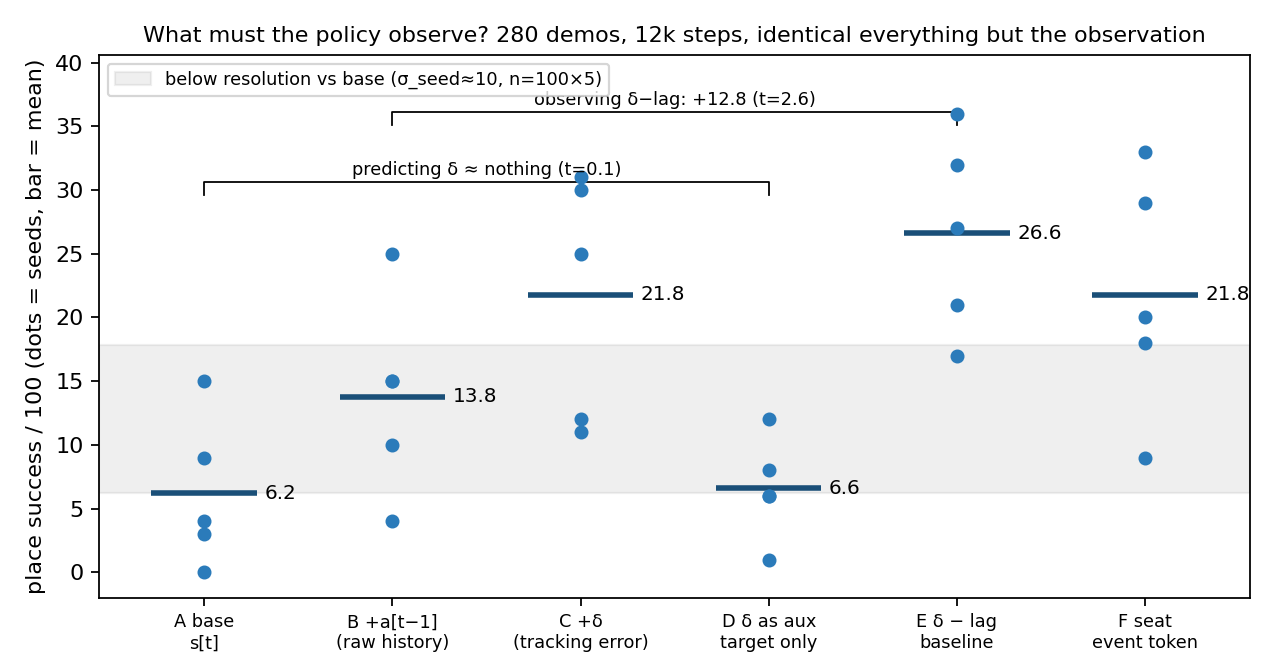
\includegraphics[width=0.85\linewidth]{fig2_grid.png}
  \caption{The observation-design grid. Bars are 5-seed means, dots
  individual seeds (100 episodes each). The gray band spans the
  below-resolution zone around base given
  $\sigma_{\text{seed}} \approx 10$. The lag-excess arm (E) is the only
  design whose margin over the history baseline (B) exceeds seed
  resolution.}
  \label{fig:grid}
\end{figure}

\subsection{Ecosystem study: a pre-registered negative}
\label{sec:corpus}

Does $\delta$ predict grasp outcomes corpus-wide? The protocol was frozen
before the run: seat detection by the stall detector of
Sec.~\ref{sec:validity}, $\delta$-at-seat as unsigned tracking error,
success proxy defined as the gripper staying closed through transport,
and the prediction that successes carry higher $\delta$ with Cohen's
$d > 0.5$ in at least 10 of 20 datasets. Of the 20 targeted
SO-100/SO-101 datasets, 16 passed the frozen inclusion gates with
connectivity: 546 episodes, 283 proxy successes.

\textbf{The prediction fails: 2/16 datasets} (pooled within-dataset
$d = -0.39$). The channel is informative with the opposite sign:
$|d| > 0.5$ in 9/16 datasets, 6/16 significantly inverted
(Fig.~\ref{fig:corpus}). The traces explain the physics. Teleop leader
devices have no hard stop, so operators over-command every close; the
seat flag fires in nearly every episode of 14/16 datasets because empty
jaws stall at the mechanical limit exactly as loaded ones do. Successful
grasps are stereotyped low-$\delta$ closes (in one dataset every clean
episode rests at the same 7-count gap), while failures carry
40--80-count frames of an operator forcing a jammed grasp. High $\delta$
at grasp time is associated with failure under the frozen proxy. This
rules out mining the corpus for success labels through this channel
alone, and it supports enforcement: the high-$\delta$ events the corpus
associates with failure are what the guard caps.

The result also bounds Sec.~\ref{sec:grid}'s transfer to retroactive
training on real teleop data. When the seat event fires in essentially
every episode, a latched seat bit (arm F) carries no information, and raw
$\delta$ at close time reads commanded depth as much as contact; what
stays informative is $\delta$ magnitude and its dynamics, which is what
the inverted effect sizes measure. Whether the lag-excess form retains
its simulated advantage when trained on over-commanded human
demonstrations is an open empirical question, not a corollary. Two
caveats attach to the corpus numbers: the recorded \texttt{action} is the
leader position, which approximates but need not equal the applied
follower command, and action-to-state timing is characterized only up to
an integer-offset sweep over $k \in \{0, \dots, 5\}$, which leaves these
conclusions unchanged (the median per-dataset shift in Cohen's $d$ across
offsets is 0.12) while estimating the physical alignment at three to four
recorded frames (App.~\ref{app:impl}).

\begin{figure}[t]
  \centering
  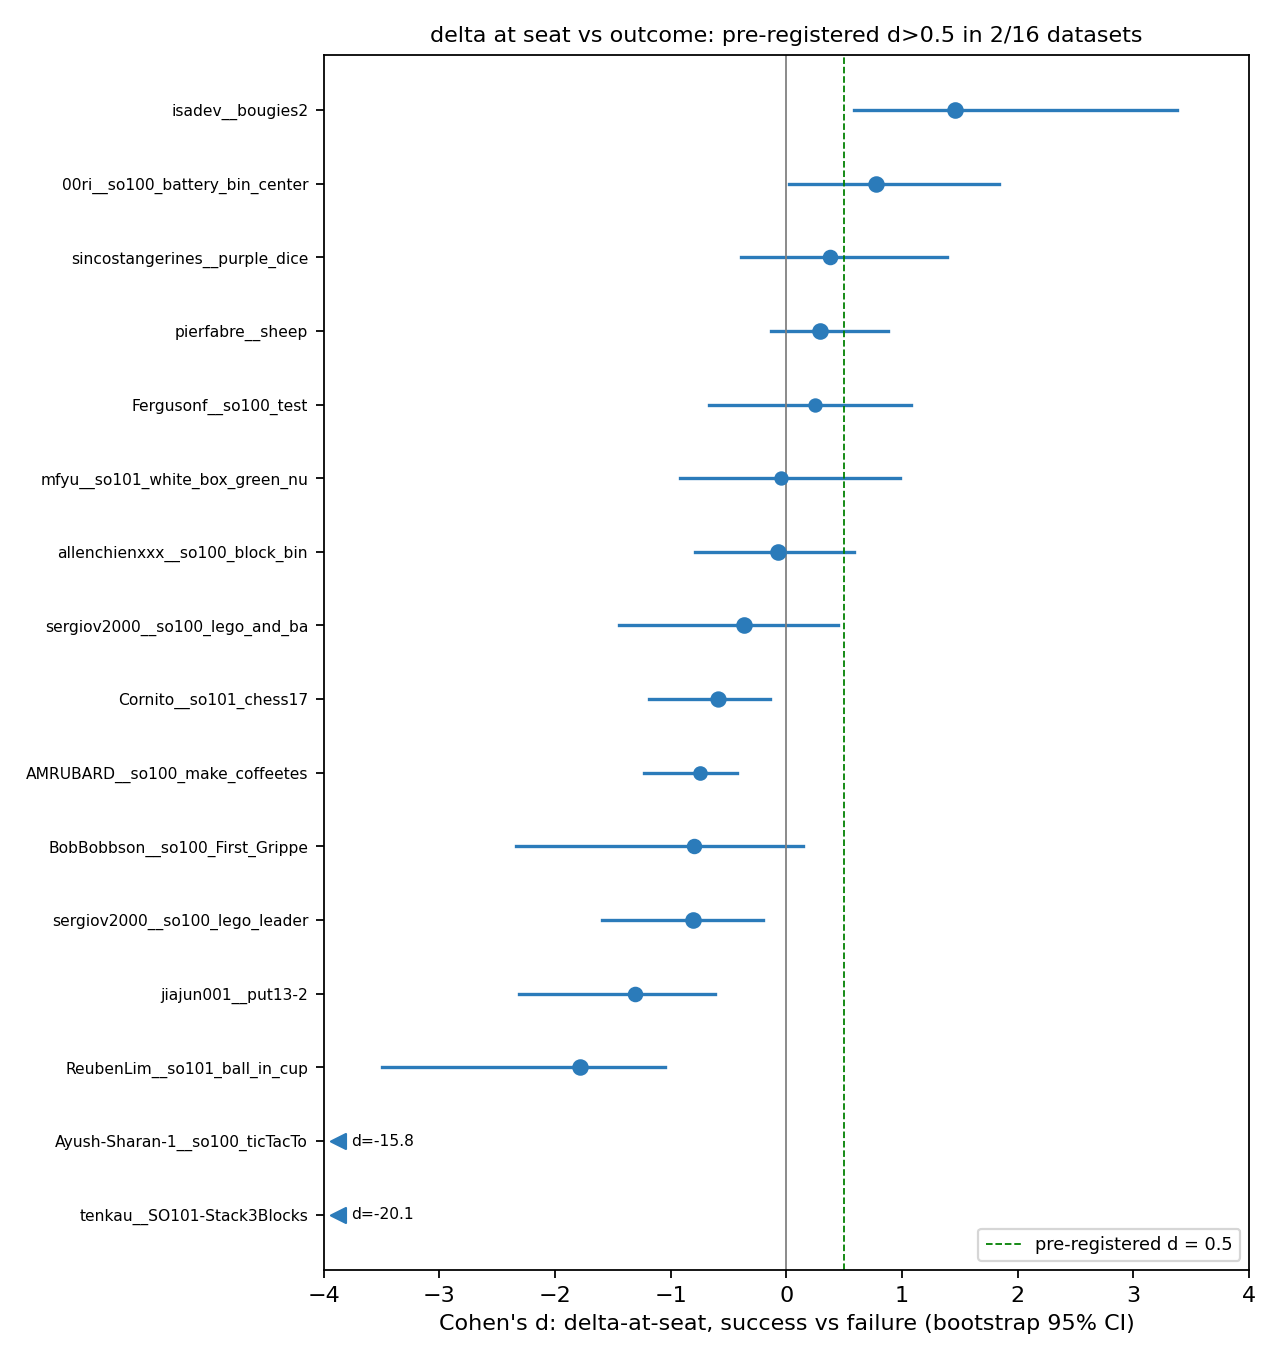
\includegraphics[width=0.85\linewidth]{fig1_corpus.png}
  \caption{Per-dataset Cohen's $d$ of $\delta$-at-seat between proxy
  successes and failures, bootstrap 95\% CIs, for the 16 datasets passing
  the frozen gates (attrition documented in the repository). Positive $d$
  was the pre-registered direction. Two datasets exceed $d = 0.5$ as
  predicted; six are significantly inverted; two task-repetitive datasets
  reach $d \approx -16$ and $-20$ because their stereotyped successes
  have near-zero $\delta$ variance.}
  \label{fig:corpus}
\end{figure}

\subsection{Runtime guard}
\label{sec:guard}

The same telemetry supports enforcement. A 40-line jaw guard (net-travel
stall and lag-excess seat detection, a 12-count squeeze budget past seat,
a closing-rate limit) runs from bus signals with no dynamics model, no
retraining, and no object knowledge; all results are simulated. Paired
against a competent scripted reference it costs about 3 placements in 30,
and on three learned checkpoints over identical paired episodes it
reduces crush events from 85 to 3 of 180 (96\%), with median peak force
dropping from 33--131\,N to 13--26\,N; it also deletes successes one
policy earned by over-gripping. Demonstrations must record applied
commands, and wrapped controllers must be closed-loop on contact.
Details, figure, and integration accounting in App.~\ref{app:guard};
bench calibration and hardware validation are in progress
(App.~\ref{app:hardware}).

%===============================================================================

\section{Limitations}
\label{sec:limitations}

All learning and guard results are simulation, on one gripper and one
object family; every quantity in newtons inherits the simulator's servo
and contact model until bench calibration lands
(App.~\ref{app:hardware}). The task is constructed to require force-band
control, so the grid measures observation design on a force-critical
task, not manipulation in general. The lag-excess model is a first-order
correction; richer free-motion predictors~\citep{oh2026factr2} may
compensate better and are untested. The seed budget leaves $C{-}B$ and
$E{-}C$ open, so the value of the subtraction itself is not established.
On real logs, $\delta$ depends on action semantics and timing that the
corpus study characterizes only up to an integer-offset sweep. The corpus
success proxy is unvalidated against ground truth, and multi-grasp tasks
were excluded by design. The channel is valid only seated and
quasi-static.

%===============================================================================

\section{Conclusion}
\label{sec:conclusion}

Position-command logs contain a retrospectively computable contact proxy:
the servo tracking error, valid within a quasi-static envelope our
simulated plant makes measurable. At 280 demonstrations, policies must
observe this channel; predicting it as the tested auxiliary target
recovers none of the gain, and the free-motion-compensated form is the
best tested instantiation. Across 16 public datasets the channel reads
operator struggle rather than success, which forecloses free outcome
labels and motivates enforcement. The open claims are the ones hardware
decides: bench calibration, retroactive training on real teleop logs, and
a copycat-style probe of when history helps versus hurts in behavior
cloning.

%===============================================================================

% \clearpage
% \acknowledgments{}

\bibliography{refs}

%===============================================================================

\clearpage
\appendix

\section{Channel computation and implementation details}
\label{app:impl}

All signals are in integer encoder counts at the recorded cadence
(stride-2 frames of a 30\,Hz bus, i.e.\ 15\,Hz):
$\delta_j[t] = a_j[t{-}1] - s_j[t]$, where $a$ is the commanded and $s$
the measured position, the $k{=}1$ alignment convention. An offset sweep
over $k \in \{0, \dots, 5\}$ on the public corpus leaves every
Sec.~\ref{sec:corpus} conclusion unchanged (the median per-dataset shift
in Cohen's $d$ across offsets is 0.12) while estimating the physical
alignment at three to four recorded frames; the bench latency measurement
(App.~\ref{app:hardware}) will pin it. The commanded rate is the first difference of commands,
$r_j[t] = a_j[t{-}1] - a_j[t{-}2]$, zero at the first two frames of an
episode. The lag model is a single per-joint scalar through the origin,
$\hat{K}_j = \sum r\delta / \sum r^2$, fit over frames whose jaw command
exceeds its 30th percentile; the jaw is the task's only contact, so
jaw-open frames are free motion. Fitted values span
$\hat{K} = 0.75$--$1.08$ across joints on our training set, computed once
on the training demonstrations and frozen. The policy input
is the concatenation
$[s_{\text{norm}},\, (\delta - \hat{K} r - \mu_\delta)/\sigma_\delta]$;
joint states and actions are standardized by dataset statistics, while
$\delta$, $e$, and the aux target use a fixed scale of
$\sigma_\delta = 8$ counts with $\mu_\delta = 0$, so no channel statistic
leaks from evaluation. The same statistics are saved beside the
checkpoint and applied identically at evaluation, where $a[t{-}1]$ is the
previously issued command, so the feature is computable from exactly what
the deployed stack already has. Appended channels concatenate onto the
state vector, leaving the network otherwise unchanged.

\section{Mechanism on a single grasp}
\label{app:mech}

\begin{figure}[h]
  \centering
  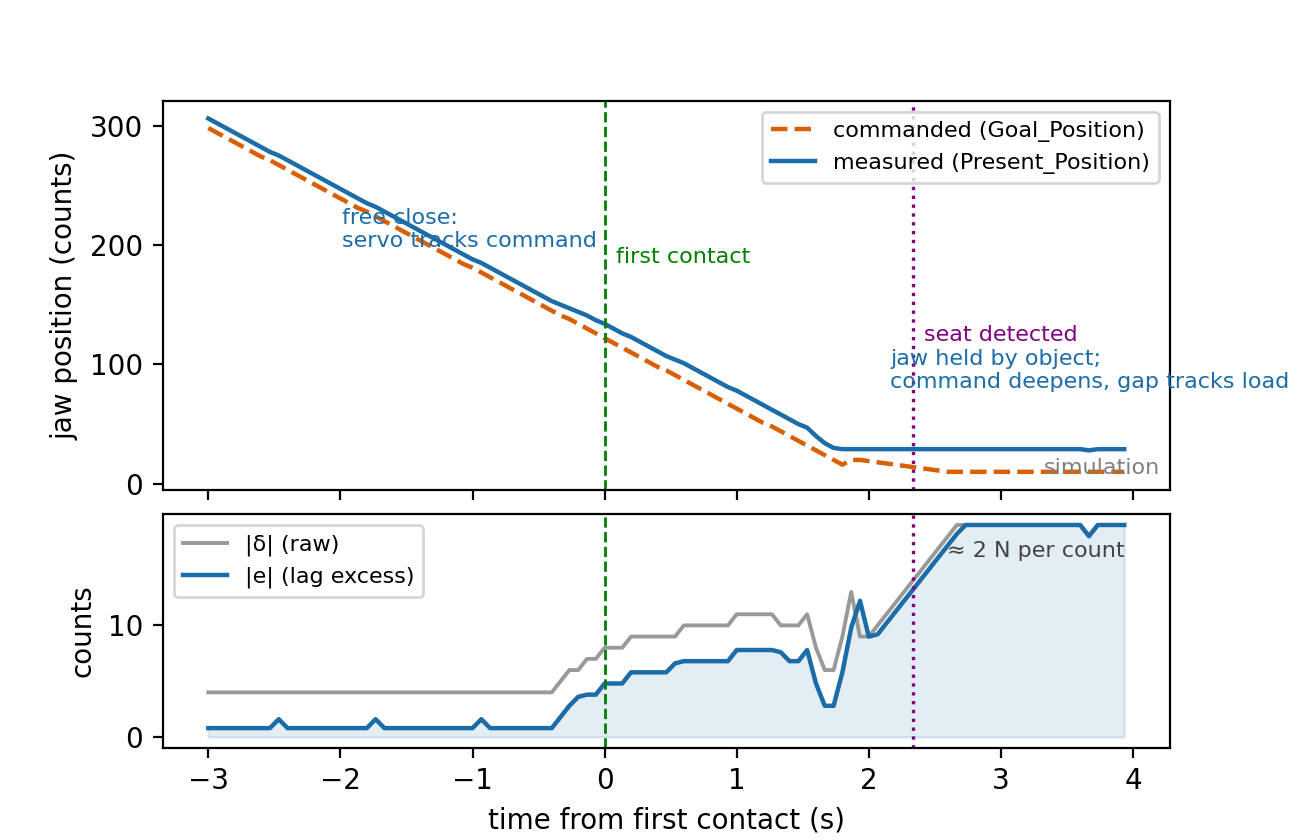
\includegraphics[width=\linewidth]{fig_mech.png}
  \caption{The channel on one servo and one grasp. The commanded position
  (dashed) and measured position (solid) track closely through the free
  close, separated only by the small following lag. At first contact
  (marked) the measured position stalls while the command continues to
  deepen; the growing gap is the load reading, $\kappa \approx 2$\,N per
  count on the simulated plant. The detector's seat event (marked) fires
  when net travel stalls while lag excess grows. The lower panel plots
  $\delta$ and the lag excess $e$ over the same frames; $e$ is near zero
  until contact by construction.}
  \label{fig:mech}
\end{figure}

\section{Guard details}
\label{app:guard}

The guard combines net-travel stall and lag-excess seat detection, a
squeeze budget of 12 counts ($\approx +24$\,N on the simulated plant)
past seat, and a closing-rate limit. Paired against a competent
reference, the scripted closed-loop teacher places 25/30 through the
guard versus 28/30 raw at a 39\,N grip (23 vs.\ 26 at the 120\,N tier).
On three learned checkpoints over identical paired episodes the guard
reduces crush events from 85 to 3 of 180 across crush tiers
(Fig.~\ref{fig:guard}), with median peak force dropping from 33--131\,N
to 13--26\,N. The guard also deletes successes a policy earned by
over-gripping: one quantized arm lifted 7/30 episodes at a 131\,N median,
and those successes vanish under the cap. Integration requires two
properties: demonstrations must record applied commands rather than
intentions, and any wrapped controller must be closed-loop on contact,
since the rate limiter breaks open-loop grasp timing by construction.
Collecting demonstrations through the guard is cost-neutral within seed
resolution on the arms measured so far.

\begin{figure}[h]
  \centering
  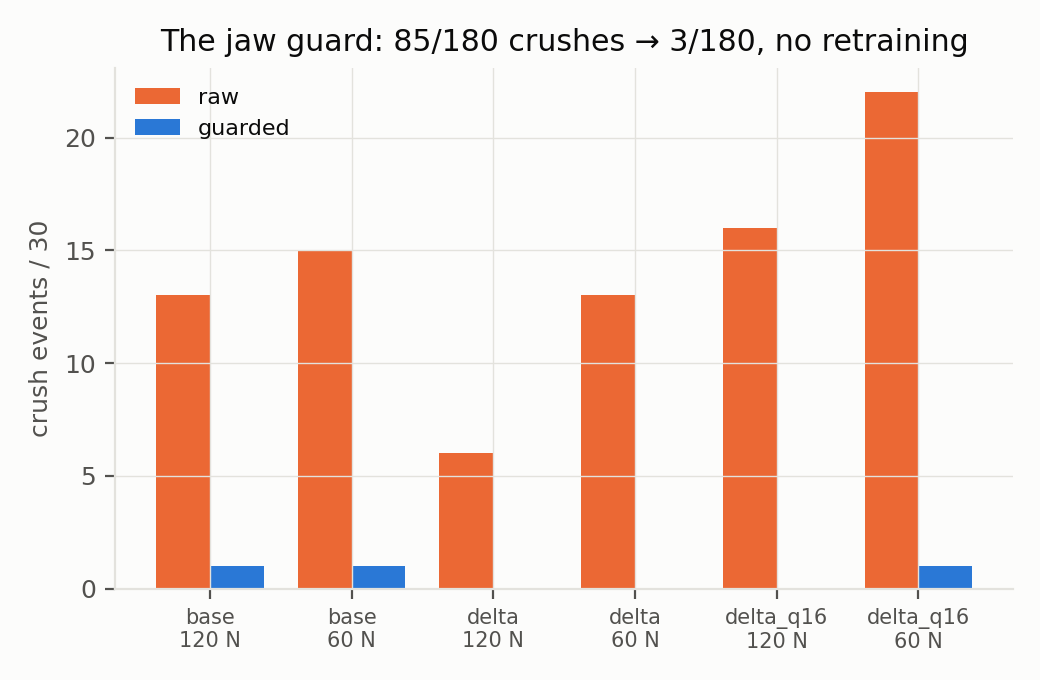
\includegraphics[width=0.75\linewidth]{fig2_guard.png}
  \caption{Crush events per 30 paired episodes for three learned
  checkpoints (base, delta, and a 16-count-quantized delta arm) at two
  crush tiers, raw (orange) versus guarded (blue). Identical checkpoints
  and episode seeds; the guard acts only through bus telemetry at
  runtime. Totals: 85 of 180 raw, 3 of 180 guarded.}
  \label{fig:guard}
\end{figure}

\section{Hardware calibration protocol (in progress)}
\label{app:hardware}

$\delta$ versus \texttt{Present\_Load}, \texttt{Present\_Current}, and a
load cell on a physical STS3215; staircase protocol at three speeds, with
opening and closing directions, repeated trials, session-start/middle/end
drift checks, and a command-to-state latency distribution measurement.
Comparison rows: the simulator's 2.0\,N/count,
\citet{hwang2018virtual}, and NeuralActuator~\citep{dou2026neuralactuator}.
Until this lands, every newton in this paper inherits the simulator's
contact model; a negative transfer result would itself be the first
measurement of the channel's sim-to-real gap.

\end{document}
